\subsection{Hojaldre}

Basada en: \href{https://elcomidista.elpais.com/elcomidista/2017/02/08/receta/1486577378_084473.html}{LA CIENCIA DE HACER HOJALDRE - El Comidista} y  \href{https://www.meilleurduchef.com/fr/recette/pate-feuilletee.html}{Pâte feuilletée - Meilleur du Chef}\\

\underline{Ingredientes}

\begin{itemize}
\item 500 gr de harina
\item 250 ml de agua
\item 10 gr de sal
\item 500 gr de mantequilla
\item Harina para espolvorear
\end{itemize}

\underline{Instrucciones}

\begin{enumerate}
\item Sacar la mantequilla del refri, o si esta afuera meterla un tiempo, tal que esté maleable pero no aguada.
\item Si la mantequilla no es un sólo bloque, amasar un poco para que todos los pedazos de integren.
\item Con ayuda de una bolsa o papel encerado, así como un rodillo y una espátula, aplanar la mantequilla hasta forme un cuadrado de \Sim 1cm de alto.
\item Mezclar la harina y la sal. Integrar el agua poco a poco.
\item Amasar un poco. La masa debe de estar homogénea pero no se necesita amasar mucho, no se necesita que esté lisa.
\item Envolver con plástico y dejar reposar por una hora a temperatura ambiente.
\item Envolver el bloque de mantequilla con la masa como se muestra en la Figura \ref{fig:envoltura-hojaldre}:
\begin{enumerate}
\item La masa de hace una bola y se hacen dos cortadas que vayan hasta mitad de la bola, tal que queden cuatro picos
\item Trabajar sobre una superfifie enharinada.
\item Los picos se extienden con un rodillo. 
\item Todo se extiende con el rodillo hasta que el cuadrado del centro tenga el tamaño de la mantequilla. Los extremos deben de tener el mismo tamaño que el centro pero más delgados.
\item Poner la mantequilla en el centro y envolver con los extremos. Cada vez que se dobla un extremo remover la harina con una brocha.
\item Cuidar que las orillas queden cerradas y cubiertas por la masa.
\end{enumerate}
\item Envolver con plástico y meter el refri durante la noche o al menos un par de horas, hasta que la masa endurezca.
\item Estirar y doblar como se muestra en la Figura \ref{fig:doblado-hojaldre} 6 veces:
\begin{itemize}
\item Si la masa esta muy dura, sobre todo la primera vez, dar uno golpecitos con el rodillo a lo largo y ancho. Es importante cuidar que la mantequilla no se separe en bolas o grumos.
\item Sobre una superficie abundantemente enharinada estirar con un rodillo en una sóla dirección hasta que tenga 3 veces lo largo (4 veces la última vez). El estirado debe de ser perpendicular a la dirección de la última vez. Es más fácil trabajar con los dobleces hacia abajo. Cuidar que los bordes queden lo más cuadrado posible.
\item Girar 90\deg y doblar en 3 (4 la última vez, haciendo primero dos dobleces al centro). El giro y el doblez tiene que ser siempre en el mismo orden --e.g. giro en sentido horario, doblar la derecha primero, izquierda después--, de tal manera que una orilla no sea siempre la que quede al último. Cada vez que se hace un doblez remover la harina con una brocha. 
\item Envolver en plástico y dejar en el refrigerador por lo menos 30 min. Si la mantequilla se está saliendo entonces es necesario dejar enfriar una hora o más.
\end{itemize}
\item Dejar en el refri por lo menos una hora antes de usarla. Se suele hornear a 200\deg - 220\deg C
\end{enumerate}

\begin{figure}
\centering
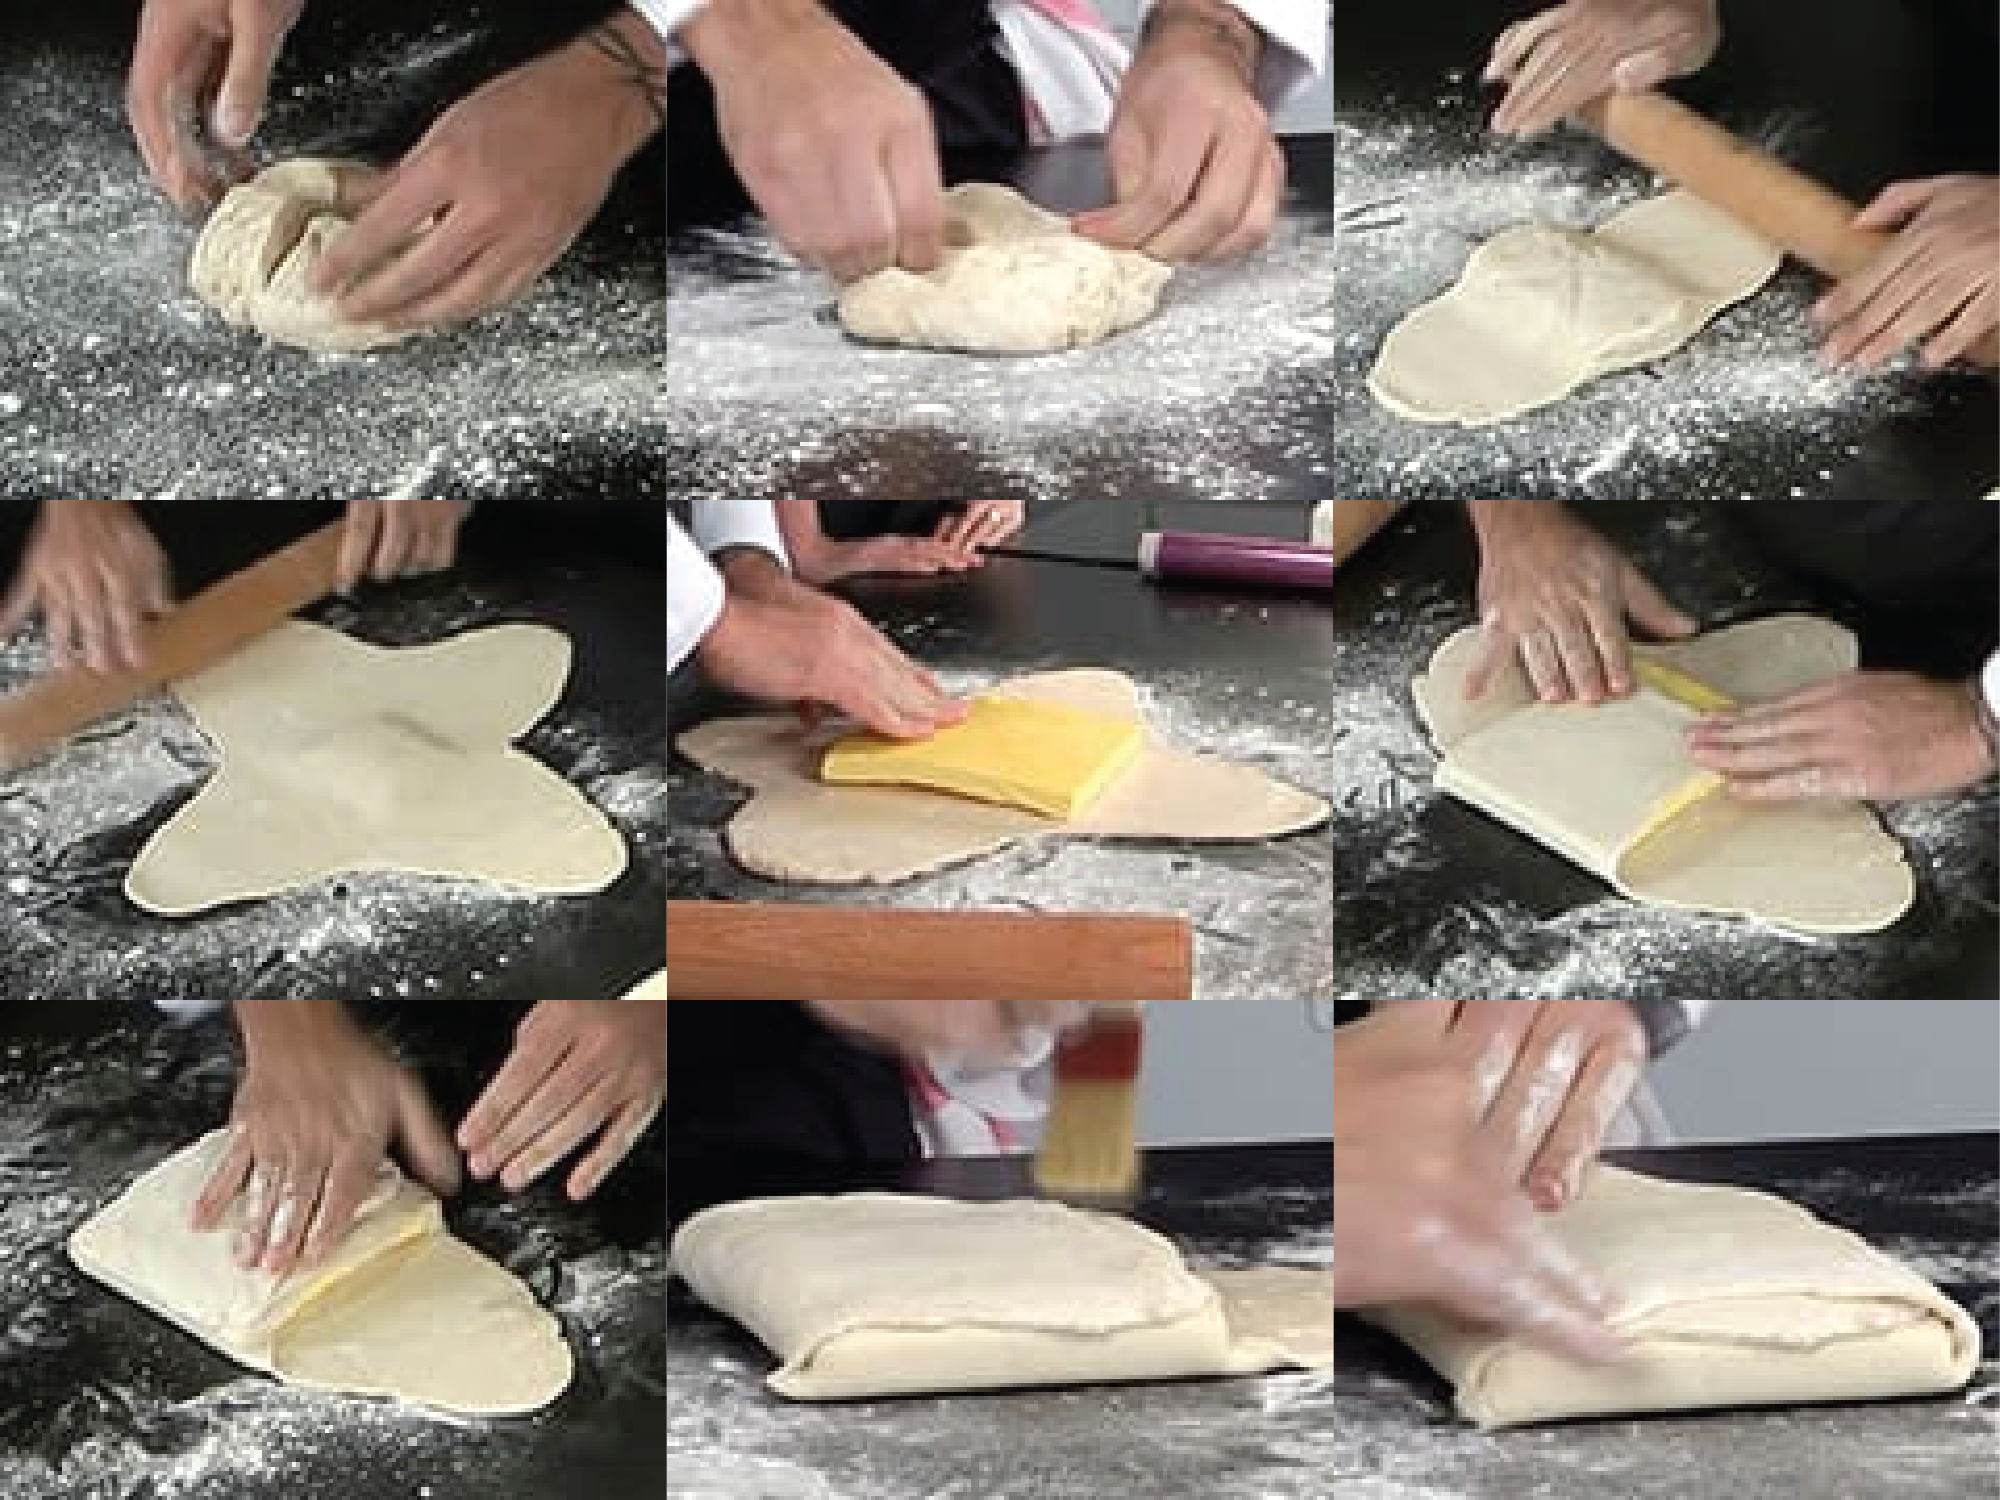
\includegraphics[width=.8\textwidth]{recetas/hojaldre/figures/envoltura.png}
\caption{Así se envuelve la mantequilla con la masa!}
\label{fig:envoltura-hojaldre}
\end{figure}

\begin{figure}
\centering
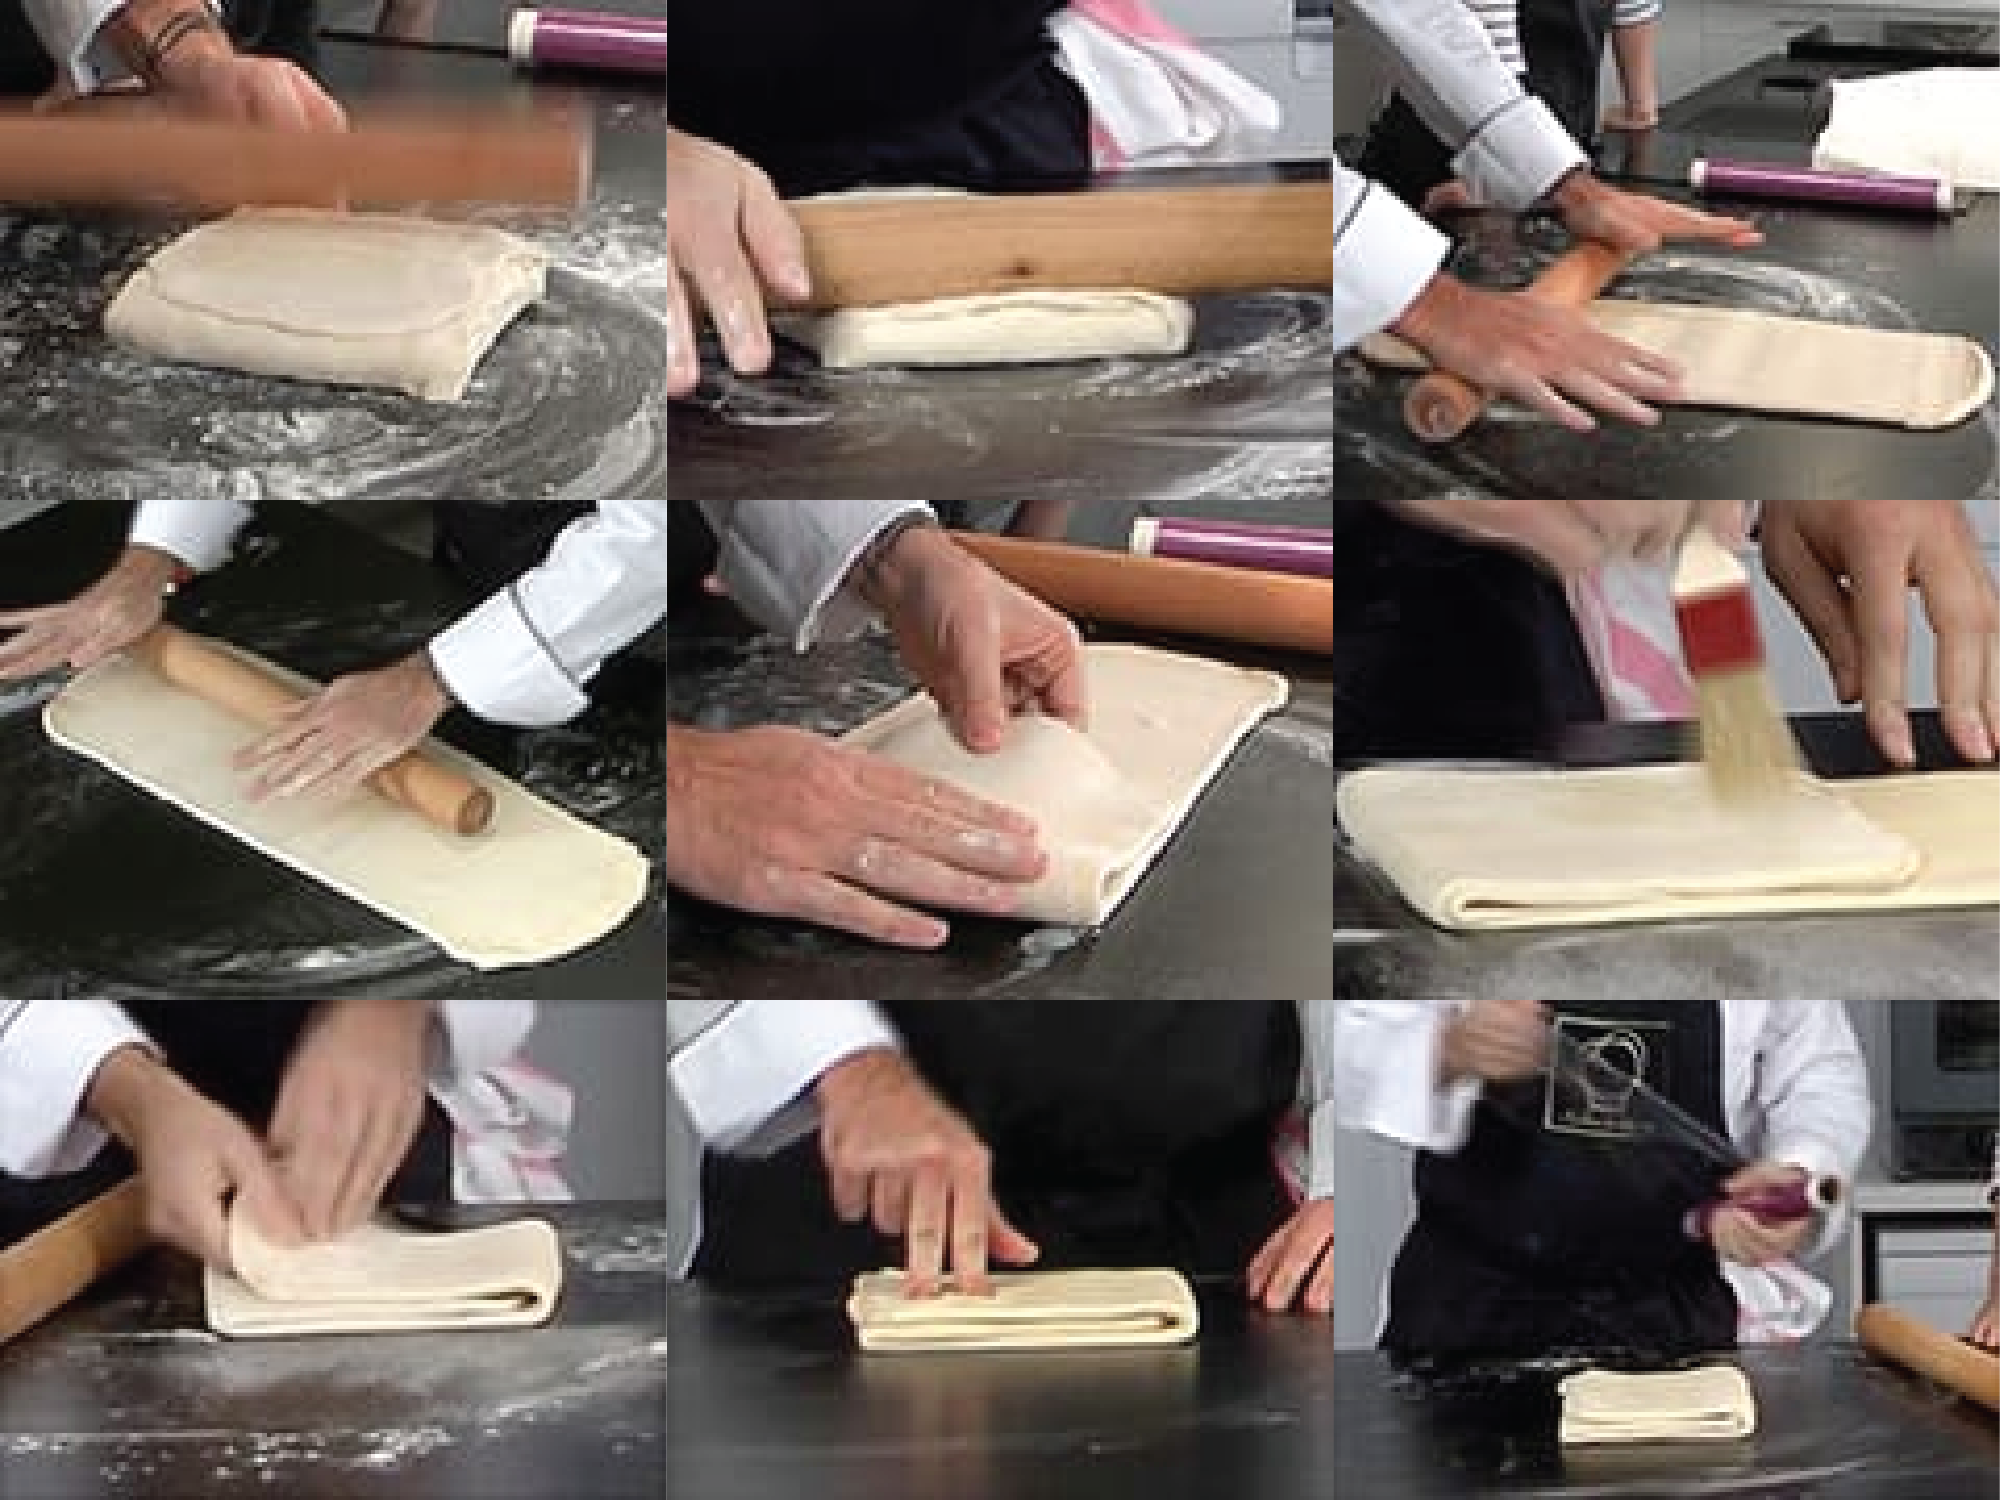
\includegraphics[width=.8\textwidth]{recetas/hojaldre/figures/doblado.png}
\caption{6 de estas!}
\label{fig:doblado-hojaldre}
\end{figure}